% =============================================================================
%  03-tutorial-diagramas-de-blocos.tex
%  Tutorial passo a passo dos diagramas de blocos de funcionamento do
%  sequencial de 6 LEDs (NE555 + CD4017B) — compilar com pdflatex (2x)
% =============================================================================
\documentclass[11pt,a4paper]{article}
\usepackage[a4paper, left=2.2cm, right=2.2cm, top=2.4cm, bottom=2.3cm,
  headheight=14pt]{geometry}
\usepackage{projeto-sabado}
\usepackage{pdflscape}
\usepackage{fancyhdr}
\usepackage{titlesec}
\usepackage{lastpage}

% =============================================================================
%  figuras/esquematico.tex — redesenho do esquemático "projeto_sabado" (Rev. 01)
%  Netlist idêntica à do print do Altium, inclusive o resistor órfão R?
%  (mantido, isolado e marcado para remoção); só a disposição foi reorganizada
%  para leitura (sinal da esquerda para a direita, VCC em cima, GND embaixo).
%
%  Uso:  \esquematico          esquemático limpo
%        \esquematico[blocos]  com as molduras tracejadas dos blocos funcionais
%  Cores de rede (sempre com rótulo textual): VCC vermelho, clock petróleo,
%  reset dourado, saídas de LED oliva; demais em preto.
% =============================================================================
\newif\ifesqblocos
\newcommand{\esquematico}[1][]{%
\esqblocosfalse
\def\esqarg{#1}\def\esqblk{blocos}%
\ifx\esqarg\esqblk\esqblocostrue\fi
\begin{circuitikz}[american, line width=0.8pt, font=\fontepino]
\ctikzset{bipoles/length=1.25cm}

% ---------------------------------------------------------------- molduras
\ifesqblocos
  \draw[moldurabloco] (-0.35,4.55) rectangle (3.75,10.55);
  \node[titulobloco, anchor=south west] at (-0.25,4.6) {1 · ALIMENTAÇÃO};
  \draw[moldurabloco] (4.0,1.55) rectangle (11.95,10.55);
  \node[titulobloco, anchor=south west] at (4.1,1.6) {2 · OSCILADOR ASTÁVEL};
  \draw[moldurabloco] (12.1,1.55) rectangle (18.15,10.55);
  \node[titulobloco, anchor=south west] at (12.2,1.6) {3 · CONTADOR + 4 · RESET (Q6)};
  \draw[moldurabloco] (18.25,1.55) rectangle (23.45,11.15);
  \node[titulobloco, anchor=south west] at (18.35,1.6) {5 · INDICAÇÃO};
\fi

% ---------------------------------------------------------------- VCC
\draw[redeVcc] (2.85,11.0) -- (15.2,11.0);
\node[rede, text=redeVcc, anchor=south west] at (2.9,11.0) {VCC};

% ---------------------------------------------------------------- 1 · ALIMENTAÇÃO
\fonteVcima[{\begin{tabular}{@{}l@{}}CR2032 · 3 V\textsuperscript{\,inf.}\\[-1pt]\scriptsize BAT-HLD-001\\[-2pt]\scriptsize (duas abas +)\end{tabular}}]{1.0}{6.3}{8.5}{\textsf{BT1}}
\draw (1.0,6.3) -- (1.0,5.6) node[ground]{};
\draw (1.0,8.5) -- (1.0,10.0) -- (1.5,10.0) node[spdt, anchor=in] (SW) {};
\node[rede, left] at (1.0,9.3) {BAT+};
\draw[redeVcc] (SW.out 1) -| (2.85,11.0);
\draw (SW.out 2) -- ++(0.35,0) coordinate (swnc);
\marcaNC{swnc}
\node[font=\fontenum, above left, inner sep=1pt] at (SW.in) {1};
\node[font=\fontenum, above, inner sep=1pt] at ($(SW.out 1)+(0.15,0)$) {2};
\node[font=\fontenum, below, inner sep=1.5pt] at (SW.out 2) {3};
\node[font=\fontepino\bfseries, anchor=north] at ($(SW.out 2)+(-0.1,-0.3)$) {SW1};
\node[font=\scriptsize\sffamily, anchor=north, text=charcoal, align=center]
  at ($(SW.out 2)+(-0.1,-0.65)$) {PCM12SMTR\\[-1pt]pinos 4–7 (MNT):\\[-1pt]sem ligação};

% ---------------------------------------------------------------- 2 · OSCILADOR (U1)
\draw[ci] (7.0,4.6) rectangle (10.0,8.6);
\pinoC{7.6}{8.6}{8}{VCC}{u1p8}
\pinoC{9.4}{8.6}{4}{$\overline{\textsf{RESET}}$}{u1p4}
\pinoE{7.0}{7.8}{7}{DISCH}{u1p7}
\pinoE{7.0}{6.6}{6}{THRES}{u1p6}
\pinoE{7.0}{5.4}{2}{TRIG}{u1p2}
\pinoD{10.0}{6.6}{3}{OUT}{u1p3}
\pinoB{7.6}{4.6}{1}{GND}{u1p1}
\pinoB{9.4}{4.6}{5}{CONT}{u1p5}
\node[align=center, font=\fontepino] at (8.75,7.35) {\textbf{U1}\\NE555DR};
% alimentação do 555 (RESET amarrado ao VCC)
\draw[redeVcc] (u1p8) -- (7.6,11.0);
\draw[redeVcc] (u1p4) -- (9.4,11.0);
\fill[redeVcc] (7.6,11.0) circle (2.2pt) (9.4,11.0) circle (2.2pt);
% rede de temporização R1-R2-C2
\draw (5.0,11.0) to[R, l_={$R_1$}, a^={\SI{1.2}{\kilo\ohm}}] (5.0,7.8);
\fill[redeVcc] (5.0,11.0) circle (2.2pt);
\draw (5.0,7.8) to[R, l_={$R_2$}, a^={\SI{10}{\kilo\ohm}}] (5.0,6.0);
\draw (5.0,6.0) to[C, l_={$C_2$}, a^={\SI{10}{\micro\farad}}] (5.0,2.8) node[ground]{};
\draw (5.0,7.8) -- (u1p7);
\draw (5.0,6.0) -- (6.0,6.0);
\draw (u1p6) -- (6.0,6.6) -- (6.0,5.4) -- (u1p2);
\node[circ] at (5.0,7.8) {};
\node[circ] at (5.0,6.0) {};
\node[circ] at (6.0,6.0) {};
\node[rede, above] at (5.75,7.8) {DIS};
\node[rede, below] at (5.5,6.0) {THR};
% GND e CONT
\draw (u1p1) -- (7.6,2.8) node[ground]{};
\draw (u1p5) to[C, l_={$C_1$}, a^={\SI{10}{\nano\farad}}] (9.4,2.8) node[ground]{};
\node[rede, right] at (9.45,3.85) {CV};

% saída do 555 -> clock do 4017 (porta OUT555 do original)
\draw[petroleo, line width=1pt] (u1p3) -- (11.8,6.6) -- (11.8,8.6) -- (13.0,8.6);
\node[rede, text=petroleo, above=1.5pt] at (11.2,6.6) {OUT555};

% ---------------------------------------------------------------- 3 · CONTADOR (U2)
\draw[ci] (13.6,3.4) rectangle (16.8,9.6);
\pinoC{15.2}{9.6}{16}{VDD}{u2p16}
\pinoE{13.6}{8.6}{14}{\hspace{2.2mm}CLK}{u2p14}
\draw[line width=0.7pt] (13.6,8.75) -- (13.82,8.6) -- (13.6,8.45);
\pinoE{13.6}{7.6}{13}{CLK INH}{u2p13}
\pinoE{13.6}{4.4}{8}{VSS}{u2p8}
\pinoB{16.0}{3.4}{15}{RESET}{u2p15}
\pinoD{16.8}{9.2}{3}{Q0}{u2q0}
\pinoD{16.8}{8.7}{2}{Q1}{u2q1}
\pinoD{16.8}{8.2}{4}{Q2}{u2q2}
\pinoD{16.8}{7.7}{7}{Q3}{u2q3}
\pinoD{16.8}{7.2}{10}{Q4}{u2q4}
\pinoD{16.8}{6.7}{1}{Q5}{u2q5}
\pinoD{16.8}{6.2}{5}{Q6}{u2q6}
\pinoD{16.8}{5.7}{6}{Q7}{u2q7}
\pinoD{16.8}{5.2}{9}{Q8}{u2q8}
\pinoD{16.8}{4.7}{11}{Q9}{u2q9}
\pinoD{16.8}{4.2}{12}{CO}{u2co}
\marcaNC{u2q7}\marcaNC{u2q8}\marcaNC{u2q9}\marcaNC{u2co}
\node[align=center, font=\fontepino] at (15.15,6.0) {\textbf{U2}\\CD4017BM96};
\draw[redeVcc] (u2p16) -- (15.2,11.0);
\draw (u2p13) -- (12.65,7.6) -- (12.65,7.0) node[ground]{};
\draw (u2p8) -- (12.65,4.4) -- (12.65,3.8) node[ground]{};

% ---------------------------------------------------------------- 4 · REALIMENTAÇÃO Q6 -> RESET
\draw[douradoEsc, line width=1pt] (u2q6) -- (17.9,6.2) -- (17.9,2.3) -- (16.0,2.3) -- (u2p15);
\node[rede, text=douradoEsc, above=2pt] at (16.85,2.3) {Q6 → RESET};

% ---------------------------------------------------------------- 5 · INDICAÇÃO (D1..D6, R3)
\foreach \q/\xj/\yl/\d in {u2q0/18.4/10.45/1, u2q1/18.9/9.45/2, u2q2/19.4/8.45/3,
                           u2q3/19.4/7.45/4, u2q4/18.9/6.45/5, u2q5/18.4/5.45/6}{
  \draw[oliva, line width=0.9pt] (\q) -| (\xj,\yl) -- (20.2,\yl);
  \draw (20.2,\yl) to[led] (21.6,\yl) -- (22.2,\yl);
  \node[font=\fontepino, anchor=south east, inner sep=1pt] at (20.15,\yl+0.04) {D\d};
}
\draw (22.2,10.45) -- (22.2,4.6) to[R, l_={$R_3$}, a^={\SI{120}{\ohm}}] (22.2,3.0) node[ground]{};
\foreach \yl in {9.45,8.45,7.45,6.45,5.45}{\node[circ] at (22.2,\yl) {};}
\node[font=\footnotesize\sffamily, text=charcoal, align=center, anchor=north]
  at (20.55,4.95) {LED verde 0805 (×6)\\[-1pt]anodo (pino 2) à esquerda};
\node[rede, right=2.5pt] at (22.2,4.85) {LED\_K};

% ---------------------------------------------------------------- resíduo do original
% resistor RES_0805C sem designador e sem ligação, como no print (deve ser apagado)
\draw (0.6,3.95) to[R] (0.6,2.35);
\marcaNC{0.6,3.95}\marcaNC{0.6,2.35}
\node[font=\fontepino, anchor=west] at (1.0,3.35) {R? (RES\_0805C)};
\node[font=\scriptsize\sffamily, anchor=west, text=redeVcc] at (1.0,2.9) {solto, sem designador:};
\node[font=\scriptsize\sffamily, anchor=west, text=redeVcc] at (1.0,2.55) {remover};
\end{circuitikz}%
}

% =============================================================================
%  figuras/blocos.tex — diagrama de blocos funcional do sequencial de LEDs
%  \diagramaBlocos                         todos os blocos em pé de igualdade
%  \diagramaBlocos[b3/.style={destaque}]   destaca o bloco 3 (usado no tutorial)
%  \diagramaBlocos[todosapagados, b2/.style={destaque}] apaga os demais
% =============================================================================
\tikzset{
  b1/.style={}, b2/.style={}, b3/.style={}, b4/.style={}, b5/.style={},
  blocofunc/.style={draw=charcoal, line width=0.8pt, rounded corners=2mm,
    fill=white, align=center, font=\footnotesize\sffamily, text width=2.75cm,
    minimum height=2.0cm, inner sep=3pt},
  destaque/.style={fill=petroleo, draw=petroleo, text=white, line width=1.3pt},
  apagado/.style={draw=charcoal!35, text=charcoal!45},
  todosapagados/.style={blocofunc/.append style={apagado}},
  sinal/.style={-{Latex[length=2.4mm]}, line width=0.95pt, draw=charcoal},
  energia/.style={dashed, line width=0.9pt, draw=redeVcc},
  rotsinal/.style={font=\footnotesize\sffamily, align=center, inner sep=1.5pt},
}
\newcommand{\diagramaBlocos}[1][]{%
\begin{tikzpicture}[#1]
  \node[blocofunc, b1] (b1) at (0,0)
    {\textbf{1 · Alimentação}\\BT1 (CR2032)\\SW1 liga/desliga};
  \node[blocofunc, b2] (b2) at (4.5,0)
    {\textbf{2 · Oscilador}\\U1 NE555\\astável\\$f\approx\SI{6,8}{\hertz}$};
  \node[blocofunc, b3] (b3) at (9.0,0)
    {\textbf{3 · Contador}\\U2 CD4017B\\Johnson +\\decodificador};
  \node[blocofunc, b5] (b5) at (13.5,0)
    {\textbf{5 · Indicação}\\D1–D6 + R3\\um LED aceso\\por vez};
  \node[blocofunc, b4, minimum height=1.25cm, text width=3.9cm] (b4) at (9.0,-2.75)
    {\textbf{4 · Realimentação}\\Q6 $\rightarrow$ RESET (módulo 6)};
  % ---------------- energia (tracejado): VCC distribuído a U1 e U2
  \draw[energia] (b1.north) -- ++(0,0.55) coordinate (e0) -- (e0 -| b3.north);
  \draw[energia, -{Latex[length=2mm]}] (e0 -| b2.north) -- (b2.north);
  \draw[energia, -{Latex[length=2mm]}] (e0 -| b3.north) -- (b3.north);
  \node[rotsinal, text=redeVcc, above] at ($(e0)!0.5!(e0 -| b2.north)$) {VCC $\approx$ \SI{3}{\volt}};
  % ---------------- sinais
  \draw[sinal] (b2) -- node[rotsinal, above] {CLK} node[rotsinal, below] {OUT555} (b3);
  \draw[sinal] (b3) -- node[rotsinal, above] {Q0…Q5} node[rotsinal, below] {1 de 6} (b5);
  \draw[sinal] ([xshift=7mm]b3.south) -- node[rotsinal, right] {Q6} ([xshift=7mm]b4.north);
  \draw[sinal] ([xshift=-7mm]b4.north) -- node[rotsinal, left] {RESET} ([xshift=-7mm]b3.south);
\end{tikzpicture}}

% =============================================================================
%  figuras/ne555-interno.tex — modelo funcional interno do 555 (didático)
%  Divisor de três resistores iguais, dois comparadores, flip-flop S-R,
%  estágio de saída e transistor de descarga. Pinos com a ligação externa
%  usada no projeto_sabado.
% =============================================================================
\newcommand{\neInterno}{%
\begin{circuitikz}[american, line width=0.8pt, font=\fontepino]
\ctikzset{bipoles/length=0.95cm}
% contorno do CI
\draw[ci, rounded corners=1.5mm, fill=douradoClaro!60] (3.0,0.4) rectangle (11.2,8.6);
\node[font=\fontepino\bfseries, anchor=south west, text=charcoal] at (6.2,0.5) {NE555 (U1)};
% pinos
\draw (3.8,8.6) -- (3.8,9.2) node[above, font=\fontepino, align=center] {8 VCC\\[-1pt]\scriptsize alimentação};
\draw (5.4,8.6) -- (5.4,9.2) node[above, font=\fontepino, align=center] {6 THRES\\[-1pt]\scriptsize ← nó THR};
\draw (8.3,8.6) -- (8.3,9.2) node[above, font=\fontepino, align=center] {4 $\overline{\textsf{RESET}}$\\[-1pt]\scriptsize ← VCC};
\draw (3.8,0.4) -- (3.8,-0.2) node[below, font=\fontepino, align=center] {1 GND\\[-1pt]\scriptsize referência};
\draw (5.4,0.4) -- (5.4,-0.2) node[below, font=\fontepino, align=center] {2 TRIG\\[-1pt]\scriptsize ← nó THR};
\draw (3.0,5.6) -- (2.4,5.6) node[left, font=\fontepino, align=right] {5 CONT\\[-1pt]\scriptsize → C1 → GND};
\draw (11.2,6.1) -- (11.8,6.1) node[right, font=\fontepino, align=left] {3 OUT\\[-1pt]\scriptsize → CLK de U2};
\draw (11.2,2.8) -- (11.8,2.8) node[right, font=\fontepino, align=left] {7 DISCH\\[-1pt]\scriptsize ← nó DIS};
% divisor interno
\draw (3.8,8.6) to[R, l_={$R$}] (3.8,5.6) to[R, l_={$R$}] (3.8,3.0) to[R, l_={$R$}] (3.8,0.4);
\node[circ] at (3.8,5.6) {};
\node[circ] at (3.8,3.0) {};
\node[font=\scriptsize\sffamily, anchor=south] at (4.45,5.62) {$2V_{CC}/3$};
\node[font=\scriptsize\sffamily, anchor=south] at (4.45,3.02) {$V_{CC}/3$};
% comparador A (limiar): + = THRES, - = 2/3 VCC
\node[op amp, noinv input up, scale=0.8] (cA) at (6.6,6.1) {};
\draw (5.4,8.6) |- (cA.+);
\draw (3.8,5.6) -| ($(cA.-)+(-0.35,0)$) -- (cA.-);
\node[font=\footnotesize\sffamily, above, text=charcoal] at (6.7,6.75) {comp. A (limiar)};
% comparador B (disparo): + = 1/3 VCC, - = TRIG
\node[op amp, noinv input up, scale=0.8] (cB) at (6.6,2.5) {};
\draw (3.8,3.0) -| ($(cB.+)+(-0.35,0)$) -- (cB.+);
\draw (5.4,0.4) |- (cB.-);
\node[font=\footnotesize\sffamily, below, text=charcoal] at (6.7,1.85) {comp. B (disparo)};
% flip-flop S-R
\draw[line width=0.9pt, fill=white] (8.0,1.9) rectangle (9.3,6.7);
\node[font=\fontepino\bfseries, rotate=90] at (8.65,4.3) {flip-flop S-R};
\draw (cA.out) -- (8.0,6.1);  \node[font=\scriptsize\sffamily, right] at (8.0,6.1) {R};
\draw (cB.out) -- (8.0,2.5);  \node[font=\scriptsize\sffamily, right] at (8.0,2.5) {S};
\node[font=\scriptsize\sffamily, left] at (9.3,6.1) {$Q$};
\node[font=\scriptsize\sffamily, left] at (9.3,2.5) {$\overline{Q}$};
\draw (8.3,8.6) -- (8.3,6.85);
\draw[fill=white] (8.3,6.78) circle (0.08);
% estágio de saída (buffer)
\draw (9.3,6.1) -- (9.7,6.1);
\draw[line width=0.9pt, fill=white] (9.7,5.75) -- (9.7,6.45) -- (10.45,6.1) -- cycle;
\draw (10.45,6.1) -- (11.2,6.1);
\node[font=\footnotesize\sffamily, above, text=charcoal] at (10.05,6.45) {saída};
% transistor de descarga
\node[npn, scale=0.85] (Qd) at (10.2,1.75) {};
\draw (9.3,2.5) -- (9.55,2.5) |- (Qd.B);
\draw (Qd.C) |- (11.2,2.8);
\draw (Qd.E) -- ++(0,-0.15) node[ground, scale=0.8]{};
\node[font=\footnotesize\sffamily, anchor=east, text=charcoal] at (9.45,1.0) {descarga};
\end{circuitikz}}

% =============================================================================
%  figuras/cd4017-interno.tex — modelo funcional do CD4017B (didático)
%  Condicionamento de clock (Schmitt) -> contador Johnson de 5 estágios
%  (realimentação pelo complemento do último estágio) -> decodificador 1-de-10.
%  Modelo lógico equivalente; a implementação interna do fabricante pode
%  usar portas diferentes com o mesmo comportamento externo.
% =============================================================================
\tikzset{
  ffj/.style={draw=charcoal, line width=0.8pt, fill=white, minimum width=0.95cm,
    minimum height=1.05cm, font=\footnotesize\sffamily, align=center, inner sep=1pt},
  blk/.style={draw=charcoal, line width=0.9pt, fill=white, rounded corners=1.5mm,
    align=center, font=\footnotesize\sffamily, inner sep=3pt},
  fio/.style={-{Latex[length=2mm]}, line width=0.8pt},
}
\newcommand{\cdInterno}{%
\begin{tikzpicture}[font=\fontepino]
  % contorno do CI
  \draw[ci, rounded corners=1.5mm, fill=douradoClaro!60] (-0.4,-1.15) rectangle (12.5,3.35);
  \node[font=\fontepino\bfseries, anchor=north west, text=charcoal] at (-0.3,3.3) {CD4017B (U2)};
  % condicionamento do clock
  \node[blk, text width=2.1cm, minimum height=1.6cm] (cond) at (0.85,1.2)
    {Schmitt-trigger\\+ habilitação\\[1pt]\scriptsize avança na borda $\uparrow$ se INH = 0};
  \draw[fio] (-1.4,1.65) node[left, font=\fontepino, align=right] {14 CLK\\[-1pt]\scriptsize ← OUT555} -- (cond.west |- 0,1.65);
  \draw[fio] (-1.4,0.75) node[left, font=\fontepino, align=right] {13 CLK INH\\[-1pt]\scriptsize ← GND} -- (cond.west |- 0,0.75);
  % contador Johnson de 5 estágios
  \draw[line width=0.8pt, rounded corners=1.5mm, draw=petroleo, fill=petroleoClaro]
    (2.55,-0.25) rectangle (9.35,2.95);
  \node[font=\scriptsize\sffamily\bfseries, text=petroleo, anchor=north west] at (2.6,2.92)
    {contador Johnson de 5 estágios};
  \foreach \n/\x in {A/3.55, B/4.85, C/6.15, D/7.45, E/8.75}{
    \node[ffj] (ff\n) at (\x,1.2) {FF \n\\[-1pt]D\enspace Q};
  }
  \foreach \a/\b in {A/B, B/C, C/D, D/E}{\draw[fio] (ff\a.east) -- (ff\b.west);}
  % realimentação: complemento do estágio E volta para o D de A
  \draw[fio, douradoEsc] (ffE.north) -- ++(0,0.55) -| ($(ffA.west)+(-0.35,0)$) -- (ffA.west);
  \node[font=\scriptsize\sffamily, text=douradoEsc, above] at (7.6,2.3) {$\overline{E}\rightarrow D_A$};
  % clock interno para todos os estágios
  \draw[fio] (cond.east |- 0,0.2) -- (2.95,0.2);
  \draw[line width=0.6pt, dashed] (2.95,0.2) -- (8.75,0.2);
  \foreach \x in {3.55,4.85,6.15,7.45,8.75}{\draw[-{Latex[length=1.5mm]}, line width=0.6pt] (\x,0.2) -- (\x,0.67);}
  \node[font=\footnotesize\sffamily, below] at (5.6,0.18) {clock interno (todos os estágios)};
  % reset assíncrono
  \draw[fio, douradoEsc] (5.1,-1.9) node[below, font=\fontepino, align=center] {15 RESET ← Q6 (pino 5)\\[-1pt]\scriptsize assíncrono: força a contagem 0} -- (5.1,-0.25);
  % decodificador
  \node[blk, text width=1.75cm, minimum height=3.1cm] (dec) at (11.25,1.35)
    {decodificador\\1-de-10\\[2pt]\scriptsize 10 portas\\AND de 2\\entradas};
  \draw[line width=2.2pt, -{Latex[length=2.6mm, width=3.2mm]}] (9.35,1.2) -- node[above=2pt, font=\footnotesize\sffamily] {A…E} (dec.west |- 0,1.2);
  % saídas
  \foreach \q/\p/\y in {0/3/2.55, 1/2/2.1, 2/4/1.65, 3/7/1.2, 4/10/0.75, 5/1/0.3, 6/5/-0.15}{
    \draw[fio, oliva] (dec.east |- 0,\y) -- (12.9,\y);
    \node[font=\scriptsize\sffamily, right] at (12.9,\y) {Q\q\ (\p)};
  }
  \node[font=\scriptsize\sffamily, right, align=left, text=charcoal] at (12.9,-0.75)
    {Q7 (6), Q8 (9),\\Q9 (11): sem uso};
  % carry-out
  \draw[fio, charcoal] (8.75,-0.25) -- (8.75,-1.9) node[below, font=\fontepino, align=center] {12 CO $=\overline{E}$\\[-1pt]\scriptsize sem uso};
\end{tikzpicture}}

% =============================================================================
%  referencias.tex — fontes verificadas (datasheets lidos nos PDFs oficiais
%  em 20–21/11/2026) e trechos de especificação reutilizados no texto.
% =============================================================================

% ---------------------------------------------------------------- trechos
\newcommand{\DSbat}{tensão nominal de \SI{3}{\volt} e corte em \SI{2}{\volt};
capacidade de \SI{225}{\milli\ampere\hour} (Panasonic) a \SI{254}{\milli\ampere\hour}
(Energizer, carga de \SI{15}{\kilo\ohm} até \SI{2}{\volt}, \SI{21}{\celsius}). Essa
capacidade é especificada com dreno contínuo de cerca de \SI{0,2}{\milli\ampere}; a
resistência interna da célula nova fica perto de \SI{10}{\ohm}~\cite{cr2032pan,cr2032en,enerman}.}

\newcommand{\DSsuporte}{o suporte faz o contato positivo pelo próprio corpo metálico,
soldado em quatro ilhas laterais (duas de cada lado, no footprint recomendado); o
negativo é uma \textbf{ilha circular de cobre de \SI{18}{\milli\meter} de diâmetro na
própria placa}, sob a bateria, que precisa ficar exposta e ligada ao GND. O desenho do
fabricante é para CR2032 (o catálogo também lista a CR2025)~\cite{bathld}.}

\newcommand{\DSsw}{SPDT, \SI{300}{\milli\ampere} a \SI{6}{\volt} CC, vida mecânica de
\num{10000} ciclos e operação de \SIrange{-20}{85}{\celsius}, segundo distribuidores. O
PDF do fabricante (C\&K, hoje Littelfuse) não pôde ser lido na verificação; por isso o
terminal comum e o significado do sufixo SMTR ficam sem confirmação. A DigiKey marca a
peça como obsoleta~\cite{pcm12}.}

\newcommand{\DSneEnc}{SOIC-8 (sufixo D); o R final indica carretel de 2500 unidades. A
versão em tubo (NE555D) consta como obsoleta~\cite{ne555}.}

\newcommand{\DSne}{VCC recomendada de \SIrange{4,5}{16}{\volt}; consumo sem carga a
\SI{5}{\volt} de \SI{3}{\milli\ampere} típicos e \SI{6}{\milli\ampere} máximos com a saída
baixa (\SI{2}{\milli\ampere} e \SI{5}{\milli\ampere} com a saída alta); limiares de cerca de
$2V_{CC}/3$ (THRES) e $V_{CC}/3$ (TRIG); RESET ativo abaixo de 0,3 a \SI{1}{\volt}, e o
datasheet manda ligá-lo ao VCC quando não usado; saída de até \SI{200}{\milli\ampere};
\SI{0,01}{\micro\farad} no CONT no circuito astável de referência; desacoplamento do VCC
com cerâmico de \SI{0,1}{\micro\farad}; operação de \SIrange{0}{70}{\celsius}~\cite{ne555}.}

\newcommand{\DScdEnc}{SOIC-16 (sufixo M); o 96 indica carretel de 2500 unidades. A
versão em tubo (CD4017BM) consta como obsoleta~\cite{cd4017}.}

\newcommand{\DScd}{VDD recomendada de \SIrange{3}{18}{\volt}; avança na borda de subida
do CLOCK com CLOCK INHIBIT em nível baixo; gatilho Schmitt na entrada de clock, que aceita
bordas lentas; RESET ativo em nível alto, que leva a contagem a zero. A \SI{5}{\volt}:
clock máximo de \SI{2,5}{\mega\hertz} (mín.) e \SI{5}{\mega\hertz} (típ.), atraso
RESET\,$\to$\,saída de \SI{265}{\nano\second} típicos e \SI{530}{\nano\second} máximos,
largura mínima recomendada do pulso de reset de \SI{260}{\nano\second} e corrente
quiescente máxima de \SI{5}{\micro\ampere} a \SI{25}{\celsius}. O datasheet não tem
tabelas a \SI{3}{\volt}, só a 5, 10 e \SI{15}{\volt}~\cite{cd4017}.}

\newcommand{\DScap}{Exemplo de código: Murata GRM21BR61A106KE19 (\SI{10}{\micro\farad}
$\pm$\SI{10}{\percent}, X5R, \SI{10}{\volt})~\cite{murata}. A perda de capacitância com
tensão contínua aplicada varia de modelo para modelo e deve ser lida na curva do
fabricante.}

\newcommand{\DSres}{exemplo: Yageo série RC, RC0805 com \SI{0,125}{\watt} a
\SI{70}{\celsius} e \SI{150}{\volt} de tensão máxima de trabalho~\cite{yageo}.}

\newcommand{\DSled}{Dois LEDs 0805 do mesmo fabricante mostram a diferença que importa:
o Kingbright APT2012SGC (GaP, \SI{568}{\nano\meter}) tem Vf de \SI{2,2}{\volt} típicos e
\SI{2,5}{\volt} máximos a \SI{20}{\milli\ampere}; o APT2012ZGC (InGaN, \SI{525}{\nano\meter})
tem \SI{3,3}{\volt} típicos e \SI{4,1}{\volt} máximos. Os dois admitem \SI{25}{\milli\ampere}
contínuos~\cite{kingbright}.}

\newcommand{\DSneVcc}{\SIrange{4,5}{16}{\volt}~\cite{ne555}}
\newcommand{\DScdVdd}{\SIrange{3}{18}{\volt}~\cite{cd4017}}
\newcommand{\DSswI}{\SI{300}{\milli\ampere} a \SI{6}{\volt} CC (distribuidor)~\cite{pcm12}}
\newcommand{\DSbatI}{Capacidade especificada com dreno de $\approx$\SI{0,2}{\milli\ampere}; dreno alto reduz a capacidade útil~\cite{cr2032en,enerman}}
\newcommand{\DScmos}{LMC555: opera a partir de \SI{1,5}{\volt}; TLC555C: a partir de
\SI{2}{\volt} (a versão TLC555I só a partir de \SI{3}{\volt}); os dois consomem cerca de
\SI{180}{\micro\ampere} típicos a \SI{5}{\volt} e são pino a pino com o 555~\cite{lmc555,tlc555}}
\newcommand{\DSledcomp}{APT2012SGC $\times$ APT2012ZGC~\cite{kingbright}}
\newcommand{\DSaltium}{\cite{altium}}

% ---------------------------------------------------------------- lista
\newcommand{\listaReferencias}{%
\begingroup
\renewcommand{\section}[2]{}%
\small
\begin{thebibliography}{99}\setlength{\itemsep}{2pt}
\bibitem{video} JuliaLabs. \emph{O porquê de eu não usar IA para desenvolver meu
hardware}. YouTube, 19 nov. 2026. \url{https://www.youtube.com/watch?v=_Q3BPcyTtds}
(trechos usados: 0:00--3:21, 7:33--10:47 e 12:08).
\bibitem{ne555} Texas Instruments. \emph{xx555 Precision Timers (NA555, NE555, SA555,
SE555)}. SLFS022K, rev. mar. 2026. \url{https://www.ti.com/lit/ds/symlink/ne555.pdf}
\bibitem{cd4017} Texas Instruments. \emph{CD4017B, CD4022B Types: CMOS
Counter/Dividers}. SCHS027C, rev. fev. 2004. \url{https://www.ti.com/lit/ds/symlink/cd4017b.pdf}
\bibitem{tlc555} Texas Instruments. \emph{TLC555 CMOS Timer}. SLFS043K, rev. jan. 2026.
\url{https://www.ti.com/lit/ds/symlink/tlc555.pdf}
\bibitem{lmc555} Texas Instruments. \emph{LMC555 CMOS Timer}. SNAS558O, rev. nov. 2026.
\url{https://www.ti.com/lit/ds/symlink/lmc555.pdf}
\bibitem{hc4017} Texas Instruments. \emph{CD54HC4017, CD74HC4017: High-Speed CMOS Logic
Decade Counter/Divider with 10 Decoded Outputs}. SCHS200D, rev. out. 2003.
\url{https://www.ti.com/lit/ds/symlink/cd74hc4017.pdf}
\bibitem{attiny} Microchip. \emph{ATtiny13A Data Sheet}. DS40002307A.
\url{https://ww1.microchip.com/downloads/aemDocuments/documents/MCU08/ProductDocuments/DataSheets/ATtiny13A-Data-Sheet-DS40002307A.pdf}
\bibitem{cmosin} Texas Instruments. \emph{Implications of Slow or Floating CMOS Inputs}.
SCBA004E, rev. jul. 2021. \url{https://www.ti.com/lit/an/scba004e/scba004e.pdf}
\bibitem{bathld} TE Connectivity (Linx). \emph{Customer Drawing C-BAT-HLD-001-XX, rev.
F1: Battery Holder CR2032 Surface Mount}, 16 jul. 2026. Página do produto:
\url{https://www.te.com/en/product-BAT-HLD-001.html}
\bibitem{cr2032pan} Panasonic Energy. \emph{CR2032 Datasheet}, fev. 2026.
\url{https://energy.panasonic.com/dam/master/pdf/en/datasheet/lithium/CR2032_Datasheet_EN.pdf}
\bibitem{cr2032en} Energizer. \emph{CR2032 Ultimate Lithium: Product Datasheet}
(UltimateCR2032EU0920). \url{https://www.data.energizer.com/pdfs/ultimatecr2032EU0920.pdf}
\bibitem{enerman} Energizer. \emph{Primary Lithium Coin Handbook and Application Manual},
mai. 2026. \url{https://data.energizer.com/wp-content/uploads/2026/05/Lithium-Coin-app-manual-0526.pdf}
\bibitem{pcm12} C\&K (Littelfuse). \emph{PCM Series Subminiature Slide Switches}.
\url{https://www.ckswitches.com/media/1424/pcm.pdf} (não acessível na verificação). Dados
de distribuidor: \url{https://www.digikey.com/en/products/detail/c-k/PCM12SMTR/1640112}
\bibitem{kingbright} Kingbright. \emph{APT2012SGC} (DSAA8210, V.18B, 2025) e
\emph{APT2012ZGC} (DSAE3711, V.14B, 2021).
\url{https://www.kingbrightusa.com/images/catalog/SPEC/APT2012SGC.pdf} e
\url{https://www.kingbrightusa.com/images/catalog/SPEC/APT2012ZGC.pdf}
\bibitem{yageo} Yageo. \emph{General Purpose Chip Resistors, RC\_L Series}, V.14, nov.
2025. \url{https://yageogroup.com/content/datasheet/asset/file/PYU-RC_GROUP_51_ROHS_L}
\bibitem{murata} Murata. \emph{Reference Sheets GRM21BR61A106KE19 e GRM216R71H103KA01}.
\url{https://search.murata.co.jp/Ceramy/image/img/A01X/G101/ENG/GRM21BR61A106KE19-01.pdf}
e \url{https://search.murata.co.jp/Ceramy/image/img/A01X/G101/ENG/GRM216R71H103KA01-01.pdf}
\bibitem{altium} Altium. \emph{Multi-sheet \& Hierarchical Designs} e \emph{Project
Options (Cross References, Net Identifier Scope)}.
\url{https://www.altium.com/documentation/altium-designer/schematic/multi-sheet-hierarchical-designs}
e \url{https://www.altium.com/documentation/altium-designer/accessing-defining-managing-project-options}
\end{thebibliography}
\endgroup}


\hypersetup{pdftitle={Tutorial — diagramas de blocos do projeto\_sabado (NE555 + CD4017B)}}

\titleformat{\section}{\Large\sffamily\bfseries\color{petroleo}}{\thesection}{0.6em}{}
\titleformat{\subsection}{\large\sffamily\bfseries\color{charcoal}}{\thesubsection}{0.6em}{}
\titlespacing*{\section}{0pt}{14pt}{6pt}

\pagestyle{fancy}
\fancyhf{}
\fancyhead[L]{\small\sffamily\color{charcoal}Tutorial · diagramas de blocos · projeto\_sabado}
\fancyhead[R]{\small\sffamily\color{petroleo}Projeto técnico assistido por LLM}
\fancyfoot[L]{\scriptsize\sffamily\color{charcoal}Rev. 1.0 · 21/11/2026}
\fancyfoot[R]{\small\sffamily\thepage/\pageref{LastPage}}
\renewcommand{\headrulewidth}{0.4pt}
\renewcommand{\headrule}{\hbox to\headwidth{\color{dourado}\leaders\hrule height \headrulewidth\hfill}}
\setlist{itemsep=2pt, topsep=4pt}
\newcolumntype{L}[1]{>{\raggedright\arraybackslash}p{#1}}
\newcolumntype{Y}{>{\raggedright\arraybackslash}X}

% caixa de "o que medir"
\newtcolorbox{medir}[1][Na bancada: o que medir]{psbase, colback=white,
  colframe=oliva, boxrule=0.8pt, title={#1}}

% filme da sequência: 6 quadros, um LED aceso por quadro
\newcommand{\filmeLEDs}{%
\begin{tikzpicture}[font=\footnotesize\sffamily]
  \foreach \k in {0,...,5}{
    \pgfmathsetmacro{\yy}{-\k*0.72}
    \ifnum\k=0 \def\rotT{$t = 0$}\else\ifnum\k=1 \def\rotT{$t = T$}\else\def\rotT{$t = \k T$}\fi\fi
    \node[anchor=east] at (-0.35,\yy) {\rotT};
    \foreach \j in {0,...,5}{
      \pgfmathtruncatemacro{\aceso}{\j==\k ? 1 : 0}
      \ifnum\aceso=1
        \fill[oliva!85!green] (\j*0.9,\yy) circle (0.22);
        \draw[oliva!60!black, line width=0.6pt] (\j*0.9,\yy) circle (0.22);
        \foreach \a in {0,45,...,315}{\draw[oliva, line width=0.5pt] ($(\j*0.9,\yy)+(\a:0.29)$) -- ($(\j*0.9,\yy)+(\a:0.37)$);}
      \else
        \draw[charcoal!45, line width=0.6pt, fill=white] (\j*0.9,\yy) circle (0.22);
      \fi
    }
    \pgfmathtruncatemacro{\qq}{\k}
    \node[anchor=west, text=charcoal] at (5.05,\yy) {Q\qq\ alta $\rightarrow$ D\pgfmathparse{int(\k+1)}\pgfmathresult\ acesa};
  }
  \foreach \j in {0,...,5}{\node[text=charcoal] at (\j*0.9,0.55) {D\pgfmathparse{int(\j+1)}\pgfmathresult};}
  \node[anchor=east, text=douradoEsc] at (-0.35,-6*0.72) {$t = 6T$};
  \node[anchor=west, text=douradoEsc] at (-0.2,-6*0.72)
    {Q6 sobe por centenas de ns, aciona o RESET e a contagem volta a Q0 (D1)};
\end{tikzpicture}}

\begin{document}

\begin{tcolorbox}[enhanced, colback=petroleo, colframe=petroleo, arc=2mm,
  left=6mm, right=6mm, top=5mm, bottom=5mm]
\color{white}\sffamily
{\small TUTORIAL PASSO A PASSO}\par\vspace{2mm}
{\LARGE\bfseries Diagramas de blocos de funcionamento}\par\vspace{1mm}
{\large Sequencial de 6 LEDs com NE555 e CD4017B (\texttt{projeto\_sabado})}\par\vspace{3mm}
{\small Cada passo acende um bloco do diagrama, mostra o que entra, o que sai, como o
bloco funciona por dentro e o que medir na bancada para provar que ele está fazendo o
trabalho dele.}
\end{tcolorbox}

\noindent{\small\sffamily\color{charcoal}
Documentos do conjunto: \textbf{01} Especificação técnica · \textbf{02} Prancha
ilustrativa A3 · \textbf{03} Tutorial dos diagramas de blocos (este).\hfill Versão 1.0 — 21/11/2026}

\tableofcontents

% =============================================================================
\section{Como ler um diagrama de blocos}
% =============================================================================
Um diagrama de blocos troca componentes por \textbf{funções}. Cada retângulo responde a
uma pergunta só: “o que este pedaço do circuito faz?”. As setas dizem o que passa de um
bloco para o outro. Neste tutorial vale a seguinte convenção:

\begin{itemize}
  \item \textbf{seta cheia:} sinal (informação), como o clock ou as saídas do contador;
  \item \textbf{linha tracejada vermelha:} energia (VCC), que alimenta os CIs;
  \item \textbf{bloco preenchido em azul petróleo:} o bloco que está sendo estudado no passo.
\end{itemize}

O método para qualquer bloco é sempre o mesmo, e vale a pena fixar: \textbf{(1)} o que
entra, \textbf{(2)} o que sai, \textbf{(3)} qual regra transforma a entrada na saída,
\textbf{(4)} como provar na bancada que a regra está sendo cumprida.

% =============================================================================
\section{Passo 0 — o sistema inteiro em uma figura}
% =============================================================================
\begin{figure}[H]
\centering
\diagramaBlocos
\caption{Diagrama de blocos completo do sequencial de 6 LEDs.}
\end{figure}

\begin{center}
\small
\begin{tabularx}{\linewidth}{@{}L{2.9cm} L{3.0cm} Y L{2.9cm}@{}}
\toprule
\textbf{Bloco} & \textbf{Entra} & \textbf{Sai} & \textbf{Componentes} \\
\midrule
1 · Alimentação & energia da bateria & VCC $\approx$ \SI{3}{\volt} quando a chave está ligada & BT1, SW1 \\
2 · Oscilador & VCC & onda quadrada OUT555 de $\approx$ \SI{6,8}{\hertz} & U1, R1, R2, C2, C1 \\
3 · Contador & CLK (= OUT555) e RESET & Q0 a Q9, só uma em nível alto por vez & U2 \\
4 · Realimentação & Q6 & RESET & fio do pino 5 ao pino 15 de U2 \\
5 · Indicação & Q0 a Q5 & luz: um LED aceso por vez & D1–D6, R3 \\
\bottomrule
\end{tabularx}
\end{center}

A frase que resume tudo: \emph{o oscilador marca o ritmo, o contador decide qual LED
acende, a realimentação fecha a volta em seis passos e os LEDs mostram o resultado.}

% =============================================================================
\section{Passo 1 — bloco de alimentação}
% =============================================================================
\begin{figure}[H]
\centering
\diagramaBlocos[todosapagados, b1/.style={destaque}]
\end{figure}

\textbf{Entra:} a energia química da bateria CR2032. \textbf{Sai:} a rede VCC, que
alimenta U1 (pinos 8 e 4) e U2 (pino 16).

\textbf{Como funciona.} O suporte BAT-HLD-001 prende a bateria: o positivo encosta no
corpo metálico do suporte e o negativo encosta numa ilha de cobre redonda da própria
placa, ligada ao GND. Do positivo, a energia vai ao pino 1 da chave SW1. Com a chave na
posição de liga, segundo o símbolo do esquemático, o pino 1 (polo) se conecta ao pino 2 e
o VCC aparece; na outra posição, o polo vai ao pino 3, que não está ligado a nada, e o
circuito fica sem energia. Qual terminal é o comum no encapsulamento real ainda precisa
ser conferido no desenho do fabricante (documento 01, achado A8).

\textbf{O ponto de atenção do bloco.} A bateria entrega cerca de \SI{3}{\volt} nova e
cai até \SI{2}{\volt} no fim da vida útil. O CD4017B é especificado a partir de
\SI{3}{\volt} e o NE555 a partir de \SI{4,5}{\volt}~\cite{ne555,cd4017}. Por isso a
especificação (documento 01, achado A1) recomenda um 555 CMOS, como o LMC555, e
lembra que trocar só o 555 não resolve o contador: a versão CD74HC4017, de 2 a
\SI{6}{\volt} e com a mesma pinagem, resolve~\cite{hc4017}.

\begin{medir}
\begin{itemize}[leftmargin=*]
  \item Multímetro entre SW1-2 (ou U1-8) e GND, chave ligada: cerca de \SI{3}{\volt}
  (até \SI{3,2}{\volt} com bateria nova). Chave desligada: \SI{0}{\volt}.
  \item Se a tensão cai muito quando o circuito oscila, a bateria está no fim ou falta
  capacitor de desacoplamento (achado A2).
\end{itemize}
\end{medir}

% =============================================================================
\section{Passo 2 — bloco oscilador (NE555 astável)}
% =============================================================================
\begin{figure}[H]
\centering
\diagramaBlocos[todosapagados, b2/.style={destaque}]
\end{figure}

\textbf{Entra:} VCC. \textbf{Sai:} a onda quadrada OUT555 (pino 3), que é o clock do
contador.

\begin{figure}[H]
\centering
\neInterno
\caption{O 555 por dentro, com a ligação externa do projeto.}
\end{figure}

\subsection{O ciclo em cinco momentos}
\begin{enumerate}
  \item \textbf{Ao ligar}, C2 está descarregado (\SI{0}{\volt}). Como o pino 2 (TRIG)
  está abaixo de $V_{CC}/3$, o comparador B seta o flip-flop: a saída vai para nível
  alto e o transistor de descarga fica cortado.
  \item \textbf{Carga.} C2 carrega pelo caminho VCC $\to$ R1 $\to$ R2 $\to$ C2. A tensão
  $v_C$ sobe em exponencial.
  \item \textbf{Limiar.} Quando $v_C$ chega a $2V_{CC}/3$, o comparador A reseta o
  flip-flop: a saída cai e o transistor de descarga conduz, prendendo o pino 7 ao GND.
  \item \textbf{Descarga.} C2 descarrega pelo caminho C2 $\to$ R2 $\to$ pino 7 $\to$ GND.
  Repare que R1 continua ligado entre VCC e o pino 7: durante toda a descarga, ele
  conduz $V_{CC}/R_1 = \SI{3}{\volt}/\SI{1,2}{\kilo\ohm} = \SI{2,5}{\milli\ampere}$ direto
  para o GND, sem fazer trabalho útil.
  \item \textbf{Disparo.} Quando $v_C$ cai a $V_{CC}/3$, o comparador B seta o flip-flop
  de novo, a saída volta para nível alto e o ciclo recomeça no momento 2.
\end{enumerate}

\subsection{Os números do bloco}
Os tempos saem das fórmulas do datasheet~\cite{ne555}, com $R_1 = \SI{1,2}{\kilo\ohm}$,
$R_2 = \SI{10}{\kilo\ohm}$ e $C_2 = \SI{10}{\micro\farad}$:
\[
t_H = 0{,}693\,(R_1+R_2)\,C_2 \approx \SI{77,62}{\milli\second},\qquad
t_L = 0{,}693\,R_2\,C_2 \approx \SI{69,30}{\milli\second},
\]
\[
T = t_H + t_L \approx \SI{146,92}{\milli\second}\;\Rightarrow\; f \approx \SI{6,81}{\hertz},
\qquad D = \frac{R_1+R_2}{R_1+2R_2} \approx \SI{52,83}{\percent}.
\]
O \textbf{primeiro} nível alto, logo depois de ligar, é mais longo, porque C2 parte de
zero e não de $V_{CC}/3$: $t_{1} = (R_1+R_2)\,C_2\ln 3 \approx 0{,}112 \times 1{,}0986
\approx \SI{123,04}{\milli\second}$. Daí em diante o circuito entra no regime da tabela.

\begin{dicaprof}
Duas perguntas que caem muito sobre o 555 astável. \textbf{Por que o ciclo de trabalho
passa de 50\%?} Porque a carga passa por $R_1 + R_2$ e a descarga só por $R_2$: a carga é
sempre mais lenta. \textbf{Por que a frequência não depende de $V_{CC}$?} Porque os dois
limiares são frações fixas de $V_{CC}$: se a tensão cai, encolhe o caminho que o
capacitor precisa percorrer, mas a corrente que o carrega também cai na mesma proporção.
Os dois efeitos se compensam, e o tempo, $\tau\ln 2$, não muda.
\end{dicaprof}

\begin{medir}
\begin{itemize}[leftmargin=*]
  \item Osciloscópio no pino 2 ou 6 (são o mesmo nó): exponencial subindo e descendo
  entre cerca de \SI{1}{\volt} e \SI{2}{\volt} (com $V_{CC} = \SI{3}{\volt}$).
  \item Osciloscópio ou frequencímetro no pino 3: onda quadrada de cerca de
  \SI{6,8}{\hertz}, com nível alto ligeiramente maior que o baixo.
  \item Frequência muito acima disso: suspeite de C2 (cerâmico que perdeu capacitância
  com a tensão aplicada, achado A4). Sem oscilação: NE555 abaixo da tensão mínima (A1).
  \item Amplitude de só cerca de \SI{1,7}{\volt} no pino 3: é o NE555 a \SI{3}{\volt}.
  Ele oscila, mas esse nível alto não chega ao que o CD4017B reconhece, e o contador pode
  não avançar (A1).
\end{itemize}
\end{medir}

% =============================================================================
\section{Passo 3 — bloco contador/decodificador (CD4017B)}
% =============================================================================
\begin{figure}[H]
\centering
\diagramaBlocos[todosapagados, b3/.style={destaque}]
\end{figure}

\textbf{Entra:} o clock no pino 14 e o RESET no pino 15. \textbf{Sai:} as dez saídas
Q0 a Q9, das quais só uma fica em nível alto por vez.

\begin{figure}[H]
\centering
\resizebox{\linewidth}{!}{\cdInterno}
\caption{O CD4017B por dentro (modelo lógico equivalente).}
\end{figure}

\textbf{Como funciona.} O clock passa primeiro por um gatilho Schmitt, que limpa bordas
lentas, e por uma porta de habilitação: com CLOCK INHIBIT (pino 13) no GND, toda borda de
\textbf{subida} avança a contagem~\cite{cd4017}. A contagem fica guardada num contador
Johnson de 5 flip-flops ligados em anel, em que o último devolve o seu complemento ao
primeiro. Com 5 estágios, esse anel percorre 10 estados, e cada estado difere do vizinho
em um bit só. O decodificador olha pares de estágios vizinhos e liga exatamente uma das
dez saídas.

\begin{center}
\small
\begin{tabular}{@{}c c c c@{}}
\toprule
\textbf{Contagem} & \textbf{Estados A B C D E} & \textbf{Saída alta (pino)} & \textbf{LED} \\
\midrule
0 & 0 0 0 0 0 & Q0 (3) & D1 \\
1 & 1 0 0 0 0 & Q1 (2) & D2 \\
2 & 1 1 0 0 0 & Q2 (4) & D3 \\
3 & 1 1 1 0 0 & Q3 (7) & D4 \\
4 & 1 1 1 1 0 & Q4 (10) & D5 \\
5 & 1 1 1 1 1 & Q5 (1) & D6 \\
6 & 0 1 1 1 1 & Q6 (5) & aciona o RESET \\
\bottomrule
\end{tabular}
\end{center}

\begin{dicaprof}
Olhe a coluna dos pinos: Q0 é o pino 3, Q1 é o 2, Q5 é o 1. As saídas do 4017
\textbf{não seguem a ordem física dos pinos}. Quem roteia a placa pela ordem dos pinos
acende os LEDs fora de sequência. Confira sempre pela tabela do datasheet.
\end{dicaprof}

\begin{medir}
\begin{itemize}[leftmargin=*]
  \item Ponta lógica ou osciloscópio nos pinos 3, 2, 4, 7, 10 e 1: cada um fica alto
  durante cerca de \SI{147}{\milli\second}, um depois do outro.
  \item Pinos 6, 9 e 11 (Q7, Q8 e Q9) ficam em nível baixo: em regime, a contagem não
  passa de 6. O pino 12 (CO) não fica parado: é alto de Q0 a Q4 e baixo durante Q5, uma
  onda de período \SI{0,88}{\second}.
  \item Ao ligar, sem reset de energização, o contador pode partir de Q7 a Q9 e ficar até
  $3T \approx \SI{0,44}{\second}$ com todos os LEDs apagados. É normal.
  \item Contagem pulando passos: suspeite de clock falso causado por queda de VCC
  (falta de desacoplamento, achado A2).
\end{itemize}
\end{medir}

% =============================================================================
\section{Passo 4 — bloco de realimentação (módulo 6)}
% =============================================================================
\begin{figure}[H]
\centering
\diagramaBlocos[todosapagados, b4/.style={destaque}]
\end{figure}

\textbf{Entra:} a saída Q6 (pino 5). \textbf{Sai:} o RESET (pino 15). É um bloco sem
componente: é só um fio. Mesmo assim, é ele que decide quantos LEDs existem na sequência.

\textbf{O que acontece na sexta borda de clock}, em ordem:
\begin{enumerate}
  \item O clock sobe e o contador passa da contagem 5 para a 6: Q5 cai e Q6 sobe.
  \item Como Q6 está ligado ao RESET, o RESET sobe junto. O RESET do CD4017B é ativo em
  nível alto e assíncrono: não espera o próximo clock.
  \item O contador zera: Q0 sobe e Q6 cai. Com Q6 baixo, o RESET também cai.
\end{enumerate}
Tudo isso dura algumas centenas de nanossegundos (o atraso RESET\,$\to$\,saída é de
\SI{265}{\nano\second} típicos a \SI{5}{\volt}~\cite{cd4017}). Para o olho, D6 apaga e
D1 acende no mesmo instante. Por isso a sequência tem 6 passos e não 7: o “passo 6” existe
só por um piscar elétrico.

\begin{dicaprof}
Regra geral para o 4017: para uma sequência de $N$ passos ($N < 10$), ligue a saída
$Q_N$ ao RESET. Para 6 LEDs, $Q_6$; para 4 LEDs, $Q_4$. Com $N = 10$ não precisa
de realimentação. O datasheet mostra ainda uma versão mais robusta, com um flip-flop S-R
que garante a largura do pulso de reset (Fig.~18 do datasheet).
\end{dicaprof}

\begin{medir}
\begin{itemize}[leftmargin=*]
  \item Osciloscópio no pino 15, em disparo único pela borda de subida: um pulso de
  centenas de nanossegundos a cada \SI{0,88}{\second}. No multímetro, esse pino mostra
  \SI{0}{\volt}: o pulso é curto demais para aparecer na média.
\end{itemize}
\end{medir}

% =============================================================================
\section{Passo 5 — bloco de indicação (LEDs)}
% =============================================================================
\begin{figure}[H]
\centering
\diagramaBlocos[todosapagados, b5/.style={destaque}]
\end{figure}

\textbf{Entra:} Q0 a Q5. \textbf{Sai:} luz, sempre em um LED por vez.

\textbf{Como funciona.} Cada saída do CD4017B alimenta o anodo de um LED; os seis catodos
se juntam e vão ao GND por um único resistor, R3 (\SI{120}{\ohm}). Funciona porque o
decodificador garante que só uma saída está alta em cada instante: só um LED conduz, e o
brilho sai igual para todos. A corrente fica entre 0,5 e \SI{1,5}{\milli\ampere}, limitada
principalmente pela própria saída CMOS. Por isso o LED precisa ser de baixa tensão direta:
verde GaP, com \SI{2,2}{\volt} típicos a \SI{20}{\milli\ampere} e cerca de 1,8 a
\SI{1,9}{\volt} na corrente deste circuito~\cite{kingbright}.

\begin{figure}[H]
\centering
\filmeLEDs
\caption{A sequência quadro a quadro. Cada quadro dura um período $T\approx\SI{0,15}{\second}$.}
\end{figure}

\begin{medir}
\begin{itemize}[leftmargin=*]
  \item Multímetro sobre R3: a tensão dividida por \SI{120}{\ohm} dá a corrente do LED
  aceso. Entre 0,06 e \SI{0,18}{\volt}, a corrente fica entre 0,5 e \SI{1,5}{\milli\ampere}.
  \item Um LED que nunca acende: confira a polaridade (anodo do lado da saída do 4017) e
  a tensão direta do modelo escolhido (achado A5).
\end{itemize}
\end{medir}

% =============================================================================
\section{Passo 6 — integração: o diagrama de tempos}
% =============================================================================
Agora junte os blocos. O diagrama de tempos mostra, no mesmo eixo, a tensão no capacitor
(bloco 2), o clock, as saídas Q0 a Q5 (blocos 3 e 5) e o pulso de reset (bloco 4).

\begin{figure}[H]
\centering
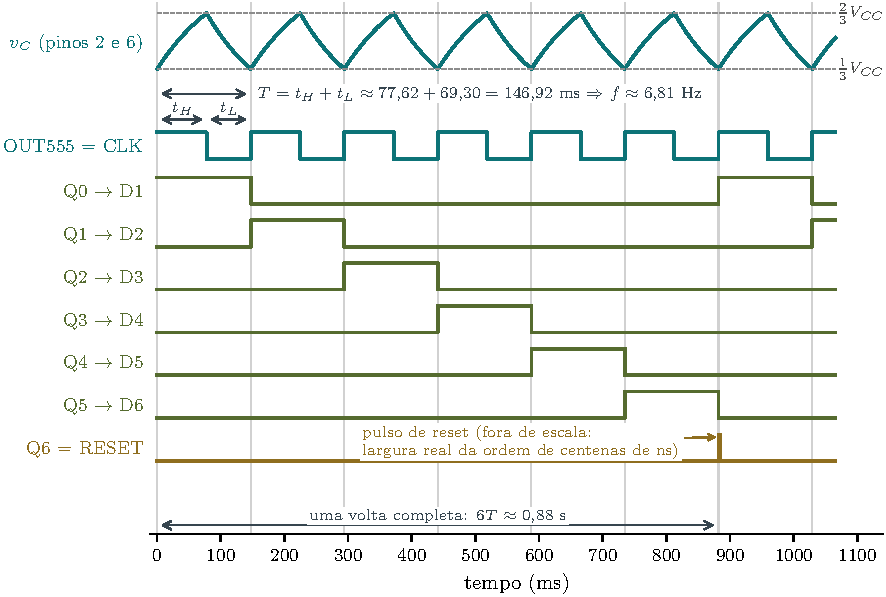
\includegraphics[width=\linewidth]{figuras/tempos-a4.pdf}
\caption{Diagrama de tempos em regime permanente (pulso de reset fora de escala).}
\end{figure}

\textbf{Como ler.} Cada linha vertical cinza é uma borda de subida do clock. Em cada
uma, uma saída do contador desce e a seguinte sobe. Siga Q0: ela fica alta de $0$ a $T$,
volta a subir em $6T$ e o ciclo se repete. A volta completa leva $6T \approx
\SI{0,88}{\second}$.

% =============================================================================
\begin{landscape}
\section{Passo 7 — do diagrama de blocos ao esquemático}
\begin{center}
\esquematico[blocos]
\end{center}
\small
\textbf{Como os blocos aparecem na folha original do Altium.} No print, a alimentação
ocupa as zonas 1A–1B, o oscilador 1C–2D, o contador 3A–3B e os LEDs 4A–4C (coluna e linha,
como na notação do Altium). A
ligação entre os blocos 2 e 3 é
feita por duas portas chamadas \texttt{OUT555}: uma no pino 3 do NE555 e outra no pino
14 do CD4017B. Portas de mesmo nome se conectam; a anotação \texttt{Sheet1[2A]} ao lado de
uma porta é a referência cruzada do Altium, que aponta a zona da folha onde está a porta
par~\cite{altium}. No redesenho acima, as portas viraram um fio direto em azul petróleo.
\end{landscape}

% =============================================================================
\section{Passo 8 — roteiro de bancada}
% =============================================================================
Na ordem em que vale a pena testar, do bloco 1 ao 5:

\begin{center}
\small
\begin{tabularx}{\linewidth}{@{}L{2.9cm} L{2.2cm} L{4.0cm} Y@{}}
\toprule
\textbf{Ponto} & \textbf{Instrumento} & \textbf{Esperado} & \textbf{Se não bater} \\
\midrule
VCC (SW1-2, U1-8, U2-16) & multímetro & $\approx$\SI{3}{\volt}; \SI{0}{\volt} com a chave desligada & bateria, chave ou contato negativo do suporte \\
U1-2/U1-6 ($v_C$) & osciloscópio & exponencial entre $\approx$1 e \SI{2}{\volt} & sem oscilação: 555 abaixo da tensão mínima (A1) \\
U1-3 (OUT555) & osciloscópio & quadrada de $\approx$\SI{6,8}{\hertz}, $D\approx\SI{53}{\percent}$ & frequência alta: C2 com capacitância efetiva menor (A4); amplitude de só $\approx$\SI{1,7}{\volt}: o 4017 pode não contar (A1) \\
U2-14 (CLK) & osciloscópio & igual a U1-3 & trilha interrompida ou solda fria \\
U2-3, 2, 4, 7, 10, 1 & ponta lógica & um pulso de $\approx$\SI{147}{\milli\second} por saída, em sequência & passos pulados: desacoplamento (A2) \\
U2-15 (RESET) & osciloscópio, disparo único & pulso de centenas de ns a cada \SI{0,88}{\second} & sem pulso: ligação Q6–RESET \\
Sobre R3 & multímetro & 0,06 a \SI{0,18}{\volt} (0,5 a \SI{1,5}{\milli\ampere}) & LED invertido ou de Vf alta (A5) \\
Consumo total & multímetro em série & 3,68 a \SI{5,73}{\milli\ampere} com NE555 (estimado) & muito acima: curto ou componente invertido \\
\bottomrule
\end{tabularx}
\end{center}

\begin{resposta}[Resumo do tutorial]
\textbf{1} A bateria e a chave entregam VCC. \textbf{2} O 555 transforma VCC em clock
de $\approx$\SI{6,8}{\hertz}, carregando e descarregando C2 entre $V_{CC}/3$ e
$2V_{CC}/3$. \textbf{3} O CD4017B avança uma saída por borda de subida. \textbf{4} Q6
reseta o contador e fecha a volta em seis passos. \textbf{5} Cada saída acende um LED,
todos pelo mesmo R3, e a luz “corre” uma volta a cada \SI{0,88}{\second}.
\end{resposta}

\section*{Referências}
\addcontentsline{toc}{section}{Referências}
\listaReferencias

\end{document}
